\documentclass[11pt]{article}
\usepackage[margin=1in]{geometry}
\usepackage{amsmath,amssymb,amsthm,graphicx,hyperref,booktabs}
\newtheorem{proposition}{Proposition}
\title{A geometry-first benchmark for geodesic nets}
\author{Research note}
\date{30 October 2026}
\begin{document}
\maketitle
The input is an unweighted stationary geodesic net in a bounded planar
rectangle. No many-body Hamiltonian is selected. We establish a reflected
net family, an exact Green-function graph invariant with spectral
coefficients, grouped reflection-orbit asymptotics, and an exact
continuous length distribution with a net threshold. These results
do not establish an exact trace formula over stationary nets.

\section{Geometric input}
Let $\Omega=(0,a)\times(0,b)$. An immersed reflected net consists of
straight segments between junctions and specular reflections at the
boundary, avoiding corners. Incidental intersections do not impose a
contact event; they can alternatively be recorded as vertices with
opposite tangent pairs, which satisfy the balance law automatically.
For a fixed reflection itinerary, the functional is total length,
\[
 L_\Gamma=\sum_{e\in E(\Gamma)}\ell_e.
\]
First variation at a free interior vertex gives
$\sum_{e\ni v}T_{e,v}=0$, where each tangent points out of the vertex.
For three unit tangents this is equivalent to pairwise angles of
$120^\circ$. Free boundary reflection points give equality of incidence
and reflection angles.

Consider three edges from $u$ to $v$, represented in the unfolded
rectangle by endpoint images
\[
 v,\qquad v-(2a,2b),\qquad v-(2a,-2b).
\]
Put $r=v-u$. Their total length is
\[
 F(r)=|r|+|r-(2a,2b)|+|r-(2a,-2b)|.
\]
Folding these unfolded lines into $\Omega$ gives the reflected edges.

\begin{proposition}
If $\sqrt3a/2<b<\sqrt3a$, the unique critical relative displacement
is
\[
 r_*=(d,0),\qquad d=2a-\frac{2b}{\sqrt3}\in(0,a).
\]
The three lengths and total length are
\[
 \ell_1=d,\qquad \ell_2=\ell_3=\frac{4b}{\sqrt3},
 \qquad L_*=2a+2\sqrt3b.
\]
Both junctions satisfy the unweighted balance law.
The family has two common-translation parameters, away from
corner-hit configurations and changes of itinerary.
\end{proposition}
\begin{proof}
At $r_*$ the three unit displacement vectors are
\[
 (1,0),\qquad(-1/2,-\sqrt3/2),\qquad(-1/2,\sqrt3/2).
\]
They sum to zero. The function $F$ is convex as a sum of norms.
Its Hessian is
\[
 D^2F=\sum_e\frac{I-T_eT_e^{\mathsf T}}{\ell_e},
\]
which is positive definite at $r_*$ because the tangents are not
parallel. Convexity and strict local convexity imply uniqueness of the
minimizing displacement. Since $F$ depends only on $v-u$, common
translations produce exactly two local zero modes. Folding preserves
length and the specular law. Reversing each path gives the balance law
at the other junction.
\end{proof}

For $a=1$ and $b=3\sqrt3/4$, take
\[
 u=(1/4,b/2),\quad v=(3/4,b/2),\quad
 (\ell_1,\ell_2,\ell_3)=(1/2,3,3),\quad L_*=13/2.
\]
These paths do not hit corners. The relative Hessian is
$\operatorname{diag}(1/2,13/6)$; the full vertex Hessian has eigenvalues
$0,0,1,13/3$. Thus this is a family, not an isolated net.

\begin{center}
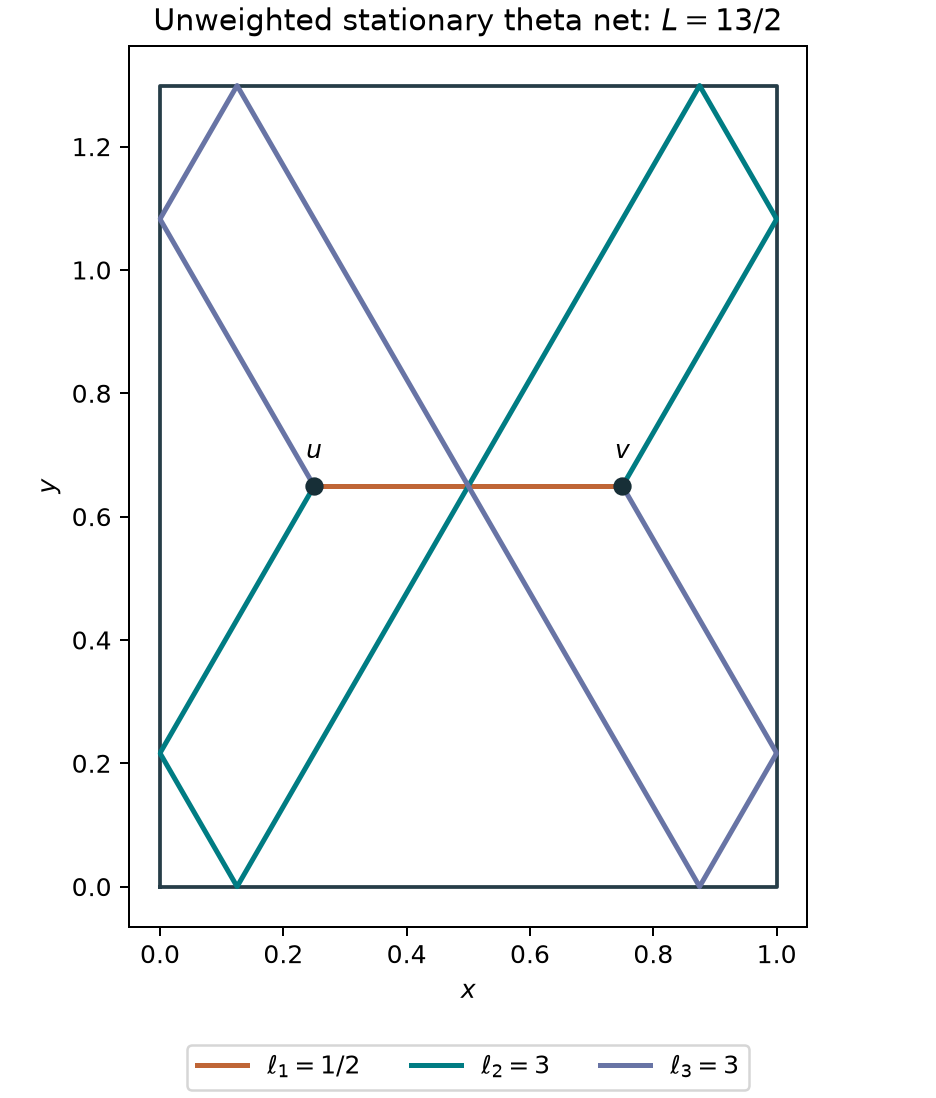
\includegraphics[width=.57\textwidth]{images/theta-net.png}
\end{center}
In this centered representative three paths meet at an incidental
crossing. The two marked vertices are the prescribed trivalent
junctions; if all intersections are recorded, the central crossing is
a balanced vertex of degree six. Translating the family generally
separates this coincidence into ordinary crossings.

\section{An exact spectral diagnostic}
Let $A=-\Delta_\Omega^D$ and let $G_\kappa$ be the kernel of
$(A+\kappa^2)^{-1}$ for $\kappa>0$. Define the theta-graph invariant
\[
 I_\theta(\kappa)=
 \int_{\Omega^2}G_\kappa(u,v)^3\,du\,dv.
\]
This is a pointwise cube of the kernel, not the trace of the cube of
the resolvent. Choose real orthonormal Dirichlet eigenfunctions
$A\phi_i=\lambda_i\phi_i$, and put
$C_{ijk}=\int_\Omega\phi_i\phi_j\phi_k$.

\begin{proposition}
In two dimensions the integral is finite, and
\[
 I_\theta(\kappa)=
 \sum_{i,j,k}
 \frac{C_{ijk}^2}
 {(\lambda_i+\kappa^2)(\lambda_j+\kappa^2)(\lambda_k+\kappa^2)}.
\]
\end{proposition}
\begin{proof}
The Dirichlet Green kernel is positive and bounded above by the
free-plane kernel $(2\pi)^{-1}K_0(\kappa|u-v|)$, whose logarithmic
diagonal singularity has an integrable cube. Regularize by
\[
 G_{\kappa,\epsilon}(u,v)=
 \sum_i\frac{e^{-\epsilon\lambda_i}\phi_i(u)\phi_i(v)}
 {\lambda_i+\kappa^2}
 =e^{\kappa^2\epsilon}\int_\epsilon^\infty
 e^{-\kappa^2t}K_t^D(u,v)\,dt.
\]
For positive $\epsilon$ expansion and integration of the cube give
the claimed nonnegative sum, with an additional factor
$e^{-\epsilon(\lambda_i+\lambda_j+\lambda_k)}$.
Spatial convergence follows by dominated convergence, since
$0\leq G_{\kappa,\epsilon}\leq e^{\kappa^2\epsilon}G_\kappa$.
The spectral sum converges by monotone convergence.
\end{proof}

The invariant uses triple eigenfunction products as well as
eigenvalues. It therefore does not establish a correspondence from
eigenvalues alone. It is also the graph contraction occurring in the
second moment of an integrated Wick cubic of a Gaussian field with
covariance $G_\kappa$: Wick pairing gives
$\mathbb E[(\int_\Omega:\!\Phi^3\!:)^2]=6I_\theta(\kappa)$.
This identifies an exact Gaussian correlation, not a chosen
fixed-particle-number Hamiltonian.

\section{Why the ordinary length functional appears}
For a reflected image path of length $\ell>0$, its resolvent factor is
\[
 g_\kappa(\ell)
 =\int_0^\infty
 \frac{e^{-\ell^2/(4t)-\kappa^2t}}{4\pi t}\,dt
 =\frac{K_0(\kappa\ell)}{2\pi}.
\]
The identity is the standard integral representation of $K_0$.
Each edge has an independently integrated time. Its exponent obeys
\[
 \min_{t>0}\left(\frac{\ell^2}{4t}+\kappa^2t\right)
 =\kappa\ell,\qquad t_*=\frac{\ell}{2\kappa}.
\]
Consequently, a graph has exponential action
$\kappa\sum_e\ell_e$, which gives the ordinary unweighted balance
law when its vertices are varied. This differs from varying vertices
with the edge times fixed. Bessel amplitudes and vertex integration
remain present at finite $\kappa$.

\begin{proposition}
For the labeled image sector specified above with
$a=1$ and $b=3\sqrt3/4$, let
\[
 B(\kappa)=\int_{\Omega^2}
 g_\kappa(|v-u|)
 g_\kappa(|v-u-(2,2b)|)
 g_\kappa(|v-u-(2,-2b)|)\,du\,dv.
\]
Then
\[
 B(\kappa)\sim
 \frac{3}{32\sqrt{13\pi}}\,
 \kappa^{-5/2}e^{-13\kappa/2}
 \qquad(\kappa\longrightarrow\infty).
\]
\end{proposition}
\begin{proof}
Writing $r=v-u$ integrates out common translation:
\[
 B(\kappa)=\int_{-1}^1\int_{-b}^b
 (1-|r_x|)(b-|r_y|)
 \prod_{e=1}^3g_\kappa(\ell_e(r))\,dr_y\,dr_x.
\]
The unique minimum of the exponent is $r_*=(1/2,0)$.
Near it all three lengths are positive, so
$K_0(z)\sim\sqrt{\pi/(2z)}e^{-z}$ applies uniformly.
The overlap weight at the minimum is $b/2$; its continuity is
sufficient for the leading Laplace term. The Hessian determinant is
$13/12$, and the product of the three edge lengths is $9/2$.
Multiplying the three Bessel prefactors by the two-dimensional
Laplace factor gives
\[
 \frac{(b/2)}{8\sqrt{2\pi}\,
       \sqrt{(13/12)(9/2)}}=\frac{3}{32\sqrt{13\pi}}.
\]
Outside a neighborhood of the minimum, strict convexity gives an
exponential gap. The other kernel singularity at $r=0$ is logarithmic
and locally integrable, so it does not change the leading term.
\end{proof}

This proposition concerns one labeled reflected-image sector. It
does not prove its coefficient survives grouping all signed
Dirichlet image sectors. Nor does it replace the full vertex
integrals by a sum over stationary nets.

\section{Reproducible numerical evidence}
Run \texttt{scripts/geodesic\_first.py}; the numerical output is in
\texttt{research-data/geodesic-first/results.json}.
Four rectangles and three optimizer initializations in each recover
the algebraic stationary displacement. The largest displacement
error is below $4\cdot10^{-8}$; angle and force residuals are at
floating-point precision. Independent edge-time quadrature and the
Bessel representation differ by at most $1.4\cdot10^{-17}$.

For the single-sector proposition, the ratio of direct numerical
integration to the predicted leading asymptotic is
\[
\begin{array}{c|rrrrr}
\kappa&10&30&100&300&1000\\ \hline
\text{ratio}&.67361&.89005&.96430&.97787&.98735
\end{array}
\]
This is evidence for the proved limit; the leading expression is
not exact at finite parameter.

For the full invariant at $\kappa=3$, reflected-image randomized
cubature gives approximately $0.000800622$, with empirical standard
error $6.9\cdot10^{-8}$. Positive spectral partial sums for coordinate
cutoffs $8,16,32,64$ are respectively
\[
 .000652957,\quad .000745879,\quad .000782625,\quad .000795134.
\]
The spectral tail remains visible and is not certified numerically.
Increasing the image winding cutoff from three to four changes one
cubature replicate by less than $9\cdot10^{-15}$; this observed change
is not a rigorous image-tail bound.

\section{What the resolvent kernel means}
For either Dirichlet or Neumann boundary conditions let $A=-\Delta$.
The resolvent is simply the inverse $R_\kappa=(A+\kappa^2I)^{-1}$.
Its kernel is the function satisfying
\[
 u(x)=\int_\Omega G_\kappa(x,y)f(y)\,dy,
 \qquad (A+\kappa^2)u=f.
\]
Thus $G_\kappa(x,y)$ is the response at $x$ to a unit point source at
$y$. On an eigenfunction with eigenvalue $\lambda_i$, the inverse
multiplies by $(\lambda_i+\kappa^2)^{-1}$. The parameter $\kappa>0$
is a spectral probe; no spatially varying potential is introduced.

\section{Reflection signs: an entire specified orbit}
The following sum includes every common reflection matrix and common
lattice shift for the selected triangle of image endpoints. It is
larger than the single sector above, but does not include triples with
different reflection matrices on different edges.
Set
\[
 b_\kappa(q)=g_\kappa(|q|)
 g_\kappa(|q-(2a,2b)|)g_\kappa(|q-(2a,-2b)|),
 \quad P_\kappa(q)=\sum_{m\in\mathbb Z^2}
 b_\kappa(q+(2am_1,2bm_2)).
\]
For $S=\operatorname{diag}(s_x,s_y)$, $s_x,s_y\in\{-1,1\}$, define
\[
 J_N=\sum_S\int_{\Omega^2}P_\kappa(u-Sv)\,du\,dv,\qquad
 J_D=\sum_Ss_xs_y\int_{\Omega^2}P_\kappa(u-Sv)\,du\,dv.
\]
These are exactly the common-parity orbit sums in the Neumann and
Dirichlet cubes: three Dirichlet edges each supply the character
$s_xs_y$, so their product is again $s_xs_y$.
Define the continuous periodic triangular weight
\[
 w_a(q)=a-2\operatorname{dist}(q,2a\mathbb Z).
\]
\begin{proposition}
The orbit sums have the exact representations
\[
 J_N=ab\int_{\mathbb R^2}b_\kappa(q)\,dq,\qquad
 J_D=\int_{\mathbb R^2}w_a(q_x)w_b(q_y)b_\kappa(q)\,dq.
\]
For $\sqrt3a/2<b<\sqrt3a$, put $d=2a-2b/\sqrt3$ and
$L_*=2a+2\sqrt3b$. Then
\[
 J_N\sim\frac{ab}{4\sqrt{6\pi L_*}}
 \kappa^{-5/2}e^{-\kappa L_*},
\]
and
\[
 \lim_{\kappa\to\infty}\frac{J_D}{J_N}
 =1-\frac{2d}{a}=\frac{4b}{\sqrt3a}-3.
\]
\end{proposition}
\begin{proof}
In one dimension the pushforward density of $(u,v)\mapsto u-v$ is
$a-|q|$ on $(-a,a)$. On the circle of length $2a$, its sum with the
pushforward density of $u+v$ is the constant $a$; their difference is
$w_a(q)$. Factor this calculation in the two coordinates and then
unfold the periodization. The resulting weights are continuous at
the unique minimum $q_*=(d,0)$, with values $ab$ and $(a-2d)b$.
Laplace's method gives the ratio. For the coefficient, if
$\ell=4b/\sqrt3$, the relative Hessian is
\[
 H=\operatorname{diag}\left(\frac{3}{2\ell},
 \frac1d+\frac1{2\ell}\right),\qquad
 (\det H)d\ell^2=\frac{3L_*}{4}.
\]
Insert this in the Bessel and Laplace prefactors computed above.
\end{proof}

In the previously selected rectangle $a=1$, $b=3\sqrt3/4$, the leading
Dirichlet coefficient cancels exactly. This is a cancellation between
families of equal length, not a failure of the junction condition.
The next term is nonzero:
\[
 J_N\sim\frac{3}{16\sqrt{13\pi}}\kappa^{-5/2}e^{-13\kappa/2},
 \qquad
 \frac{J_D}{J_N}=\frac{20}{39\kappa}+O(\kappa^{-3/2}).
\]
To check the second formula directly, write
$F=\sum_e\ell_e$ and $A_0=(\ell_1\ell_2\ell_3)^{-1/2}$.
For the positive Laplace weight $A_0e^{-\kappa F}$, expansion about
$q_*=(1/2,0)$ gives
\[
 \mathbb E[q_x-1/2]=\frac{\mu_x}{\kappa}+O(\kappa^{-2}),
 \quad
 \mu_x=(H^{-1}\nabla\log A_0)_x
 -\frac12\sum_{i,j,k}(H^{-1})_{xi}F_{ijk}(H^{-1})_{jk}.
\]
Here $\partial_x\log A_0=-5/6$, $F_{xxx}=1/4$,
$F_{xyy}=-149/36$, and $H^{-1}=\operatorname{diag}(2,6/13)$.
Consequently $\mu_x=-5/3+55/39=-10/39$.
Locally $w_1(q_x)=-2(q_x-1/2)$ and
$w_b(q_y)=b-2|q_y|$. The latter cusp contributes only at the stated
smaller order, since its first product with the leading odd
$q_x-1/2$ integrand integrates to zero. This yields $20/39$.
The $O(\kappa^{-1})$ Bessel amplitude correction does not change this
first nonzero mean: its constant term cancels on normalization.

\section{An exact length distribution with a net threshold}
The Neumann orbit above admits an exact positive length-side
representation. The standard Bessel identity gives
\[
 g_\kappa(\ell)=\frac1{2\pi}
 \int_\ell^\infty\frac{e^{-\kappa s}}{\sqrt{s^2-\ell^2}}\,ds.
\]
Define $h_\ell(s)=\mathbf1_{\{s>\ell\}}(s^2-\ell^2)^{-1/2}$ and
the positive measure, with its locally integrable density,
\[
 \rho_N(s)=\frac{ab}{(2\pi)^3}
 \int_{\mathbb R^2}
 (h_{\ell_1(q)}*h_{\ell_2(q)}*h_{\ell_3(q)})(s)\,dq.
\]
Values at the finitely many points where an individual $\ell_e=0$
can be omitted; the joint integral defines the density almost everywhere.
Tonelli's theorem proves the exact identity
\[
 J_N(\kappa)=\int_0^\infty e^{-\kappa s}\rho_N(s)\,ds.
\]
The density vanishes for $s<L_*$, because the convolution requires
$s\geq\sum_e\ell_e(q)\geq L_*$. It is positive for $s>L_*$.
Thus the geometry gives the exact lower endpoint of this orbit's
length distribution, not just an approximate exponential rate.
For $a=1$, $b=3\sqrt3/4$, local expansion at the minimum gives
\[
 \rho_N(s)\sim\frac{1}{4\pi\sqrt{13}}
 (s-13/2)^{3/2}\quad\text{as }s\downarrow13/2.
\]
Indeed each edge density is asymptotic to
$(2\ell_e)^{-1/2}(s-\ell_e)^{-1/2}$. Their convolution is a beta
integral, and integration over the positive quadratic relative
Hessian supplies one more power. Equivalently the coefficient is
the previously derived $3/(16\sqrt{13\pi})$ divided by
$\Gamma(5/2)$; the local convolution argument, not a Tauberian
inference alone, justifies the pointwise threshold asymptotic.
This is not a discrete exact sum over stationary nets. It is an exact
continuous length measure with a threshold determined by the net.

\section{Additional numerical checks}
The script \texttt{scripts/net\_reflection\_signs.py} checks the orbit
formulas in four aspect ratios. At $\kappa=30000$ the normalized
Neumann coefficient differs from its proved limit by about
$6.4\cdot10^{-7}$ relative, and
$\kappa J_D/J_N\approx0.52876$, approaching $20/39\approx0.51282$.
The remaining difference is consistent with the slow
$O(\kappa^{-1/2})$ correction after this rescaling.
Increasing the scaled integration box radius from $14$ to $18$ at
$\kappa=300$ changes the rescaled integrals by less than $10^{-15}$.
These are numerical controls, not certified quadrature bounds.

The entire Neumann graph invariant, including mixed-parity sectors,
also has the triple-eigenfunction expansion. Positive cosine-mode
partial sums and independent reflected-image cubature are recorded
in \texttt{research-data/geodesic-first/reflection-signs.json}.
A zero-padded convolution evaluates the same finite cosine sum using
its signed-mode selection rules. Direct tensor contraction at small
cutoffs checks this implementation independently. The spectral tail
is still not certified. Neither this numerical comparison nor the
orbit theorem determines the coefficient at this length after all
other geometric families have been combined.

An independent cubature of the exact three-edge length convolution
checks the threshold density without using a Bessel approximation.
For length excesses $0.03$, $0.01$, and $0.003$, its ratio to the
proved leading threshold expression is respectively
$0.9997689$, $0.9999230$, and $0.9999769$.
Four scrambled quasi-Monte Carlo replicates with $2^{16}$ points each
give empirical errors recorded in the results file. These remain
numerical estimates, not certified quadrature bounds.

\section{What remains open}
The geometry determines a promising graph contraction without
requiring a contact Hamiltonian. An exact stationary-net trace
formula remains unproved. The next tests should address:
whether the remaining mixed-parity image sectors alter the net's
length singularity in the full graph invariant;
whether the exact continuous length measure admits an exact
stationary-net expansion; and whether the spectral
side can be a trace of a natural operator, or necessarily includes
eigenfunction multiplication data. Hyperbolic examples have not
been computed in this test.

\begin{thebibliography}{9}
\bibitem{dlmf} NIST Digital Library of Mathematical Functions,
\href{https://dlmf.nist.gov/10.32.E10}{Equation 10.32.10}.
\end{thebibliography}
\end{document}
